\documentclass{article}

\usepackage{amsmath}
\usepackage{tikz}
\usepackage{palatino}

\begin{document}
\begin{enumerate}
\item[1.9.8]

\item[]
\item[1.9.10.1]
  The goal is to show that the limit of the two object diagram with arrows $f: A \rightarrow B$ and $g : A \rightarrow B$ is an equalizer of $f$ and $g$.
  \begin{center}
    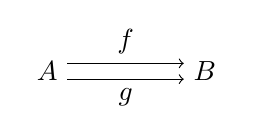
\begin{tikzpicture}
      \node (1) {$A$};
      \node [right of=1,xshift=1cm] (2) {$B$};

      \draw[transform canvas={yshift=0.1cm},->] (1) -- node[above] {$f$} (2);
      \draw[transform canvas={yshift=-0.1cm},->] (1) -- node[below] {$g$} (2);
    \end{tikzpicture}
  \end{center}
  To begin, a cone for this diagram consists of an object $X$ and arrows $a : X \rightarrow A$ and $b : X \rightarrow B$ such that the diagram commutes.
  \begin{center}
    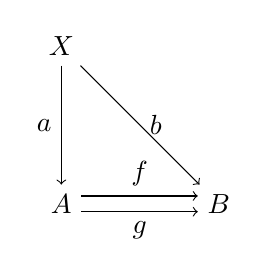
\begin{tikzpicture}
      \node (1) {$A$};
      \node [right of=1,xshift=1cm] (2) {$B$};
      \node [above of=1,yshift=1cm] (3) {$X$};

      \draw[transform canvas={yshift=0.1cm},->] (1) -- node[above] {$f$} (2);
      \draw[transform canvas={yshift=-0.1cm},->] (1) -- node[below] {$g$} (2);
      \draw[->] (3) -- node[left] {$a$} (1);
      \draw[->] (3) -- node[right] {$b$} (2);
    \end{tikzpicture}
  \end{center}
  However, $b$ is uniquely determined by the commutativity of the diagram to be the common composition $f \circ a = g \circ a$.
  (This is the same argument Pierce uses in his example of pullbacks as the limit of L-shaped diagrams.)

  \hfill{}
    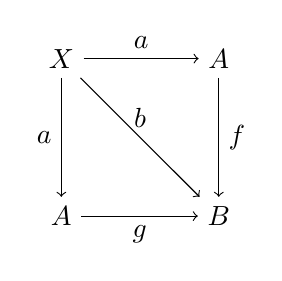
\begin{tikzpicture}
      \node (1) {$X$};
      \node [right of=1,xshift=1cm] (2) {$A$};
      \node [below of=1,yshift=-1cm] (3) {$A$};
      \node [right of=3,xshift=1cm] (4) {$B$};

      \draw[->] (2) -- node[right] {$f$} (4);
      \draw[->] (3) -- node[below] {$g$} (4);
      \draw[->] (1) -- node[above] {$a$} (2);
      \draw[->] (1) -- node[left] {$a$} (3);
      \draw[->] (1) -- node[above] {$b$} (4);
    \end{tikzpicture}
  \hfill{}
    \begin{tikzpicture}
      \node (1) {$X$};
      \node [right of=1,xshift=1cm] (2) {$A$};
      \node [below of=1,yshift=-1cm] (3) {$A$};
      \node [right of=3,xshift=1cm] (4) {$B$};

      \draw[->] (2) -- node[right] {$f$} (4);
      \draw[->] (3) -- node[below] {$g$} (4);
      \draw[->] (1) -- node[above] {$a$} (2);
      \draw[->] (1) -- node[left] {$a$} (3);
      %% \draw[->] (1) -- node[right] {$b$} (4);
    \end{tikzpicture}
  \hfill{}
  
  A limit of these diagrams has the property that any other $X'$ with an arrow $a'$ making the diagram commute has a unique arrow $k : X' \rightarrow X$.
  This gives us a commutative diagram identical to the equalizer diagram.
  Therefore our limit is an equalizer of $f$ and $g$.
  \begin{center}
    \begin{tikzpicture}
      \node (1) {$X$};
      \node[below of=1,yshift=-1cm] (2) {$X'$};
      \node [right of=1,xshift=1cm] (3) {$A$};
      \node [right of=3,xshift=1cm]  (4) {$B$};

      \draw[->] (1) -- node[above] {$a$} (3);
      \draw[dashed,->] (2) -- node[left] {$k$} (1);
      \draw[->] (2) -- node[below] {$a'$} (3);
      \draw[transform canvas={yshift=0.1cm},->] (3) -- node[above] {$f$} (4);
      \draw[transform canvas={yshift=-0.1cm},->] (3) -- node[below] {$g$} (4);
    \end{tikzpicture}
  \end{center}
  
\newpage
\item[1.9.10.2]
  The limit is the infinium $i\in \mathcal{C}$
  of the elements $D_i\in \mathcal{D}$.

  The colimit is the suprenam in $\mathcal{C}$ of
  the same elements, $D_i \in \mathcal{D}$.

\item[]
\item[1.9.10.3]
\item[]
\item[1.9.10.4]
\end{enumerate}
\end{document}
